% The comment below tells Rubber to compile the .dot files.
%
% rubber: module graphics
% rubber: rules rules.ini

\documentclass{beamer}

\usetheme{default}

\usefonttheme{structurebold}
\usepackage{helvet}
\usepackage{multimedia}         % movie
\usecolortheme{seagull}         % white on black

\usepackage[utf8]{inputenc}
\PassOptionsToPackage{hyphens}{url}\usepackage{hyperref,xspace,multicol}
\usepackage[absolute,overlay]{textpos}
\usepackage{tikz}
\usetikzlibrary{arrows,shapes,trees,shadows,positioning}
\usepackage{fancyvrb}           % for \Verb

% Remember the position of every picture.
\tikzstyle{every picture}+=[remember picture]

\tikzset{onslide/.code args={<#1>#2}{%
  \only<#1>{\pgfkeysalso{#2}} % \pgfkeysalso doesn't change the path
}}

% Colors.
\definecolor{guixred1}{RGB}{226,0,38}  % red P
\definecolor{guixorange1}{RGB}{243,154,38}  % guixorange P
\definecolor{guixyellow}{RGB}{254,205,27}  % guixyellow P
\definecolor{guixred2}{RGB}{230,68,57}  % red S
\definecolor{guixred3}{RGB}{115,34,27}  % dark red
\definecolor{guixorange2}{RGB}{236,117,40}  % guixorange S
\definecolor{guixtaupe}{RGB}{134,113,127} % guixtaupe S
\definecolor{guixgrey}{RGB}{91,94,111} % guixgrey S
\definecolor{guixdarkgrey}{RGB}{46,47,55} % guixdarkgrey S
\definecolor{guixblue1}{RGB}{38,109,131} % guixblue S
\definecolor{guixblue2}{RGB}{10,50,80} % guixblue S
\definecolor{guixgreen1}{RGB}{133,146,66} % guixgreen S
\definecolor{guixgreen2}{RGB}{157,193,7} % guixgreen S

\setbeamerfont{title}{size=\huge}
\setbeamerfont{frametitle}{size=\huge}
\setbeamerfont{normal text}{size=\Large}

% White-on-black color theme.
\setbeamercolor{structure}{fg=guixorange1,bg=black}
\setbeamercolor{title}{fg=white,bg=black}
\setbeamercolor{date}{fg=guixorange1,bg=black}
\setbeamercolor{frametitle}{fg=white,bg=black}
\setbeamercolor{titlelike}{fg=white,bg=black}
\setbeamercolor{normal text}{fg=white,bg=black}
\setbeamercolor{alerted text}{fg=guixyellow,bg=black}
\setbeamercolor{section in toc}{fg=white,bg=black}
\setbeamercolor{section in toc shaded}{fg=white,bg=black}
\setbeamercolor{subsection in toc}{fg=guixorange1,bg=black}
\setbeamercolor{subsection in toc shaded}{fg=white,bg=black}
\setbeamercolor{subsubsection in toc}{fg=guixorange1,bg=black}
\setbeamercolor{subsubsection in toc shaded}{fg=white,bg=black}
\setbeamercolor{frametitle in toc}{fg=white,bg=black}
\setbeamercolor{local structure}{fg=guixorange1,bg=black}

\newcommand{\highlight}[1]{\alert{\textbf{#1}}}

\title{GNU~Guix:\\the functional\\GNU/Linux distro\\that's a Scheme library}

\author{Ludovic Courtès}
\date{\small{Scheme Workshop\\18 September 2016, Nara, Japan}}

\setbeamertemplate{navigation symbols}{} % remove the navigation bar

\AtBeginSection[]{
  \begin{frame}
    \frametitle{}
    \tableofcontents[currentsection]
  \end{frame} 
}


\newcommand{\screenshot}[1]{
  \begin{frame}[plain]
    \begin{tikzpicture}[remember picture, overlay]
      \node [at=(current page.center), inner sep=0pt]
        {\includegraphics[width=\paperwidth]{#1}};
    \end{tikzpicture}
  \end{frame}
}


%% \usepackage{pgfpages}
%% \setbeameroption{second mode text on second screen}
%% \setbeameroption{previous slide on second screen}

\begin{document}

\maketitle

%% \begin{frame}[typeset second]
%%   This text is shown on the left and on the right.
%%   \only<second>{This text is only shown on the right.}
%%   \only<second:0>{This text is only shown on the left.}
%% \end{frame}

\setbeamercolor{normal text}{bg=white}
\begin{frame}[plain]
  \begin{tikzpicture}[remember picture, overlay]
    \node [at=(current page.center), inner sep=0pt]
          {
\includegraphics[width=0.7\paperwidth]{images/GuixSD-horizontal-print}};
  \end{tikzpicture}
\end{frame}
\setbeamercolor{normal text}{fg=white,bg=black}

\setbeamercolor{normal text}{bg=guixblue2}
\begin{frame}
  \Huge{\textbf{Functional package management.}}
\end{frame}
\setbeamercolor{normal text}{fg=white,bg=black}

\begin{frame}[fragile]

  \begin{semiverbatim}
\$ guix package -i gcc-toolchain coreutils sed grep
\textrm{...}

\$ eval `guix package --search-paths`
\textrm{...}

\$ guix package --manifest=my-software.scm
\textrm{...}
  \end{semiverbatim}

  \begin{tikzpicture}[overlay]
    \node[rounded corners=4, text centered, fill=guixorange1,
          inner sep=4mm, opacity=.75, text opacity=1,] at (current page) {
      \movie[autostart, externalviewer]{\Large{$\blacktriangleright$}}{https://audio-video.gnu.org/video/misc/2016-07__GNU_Guix_Demo_2.webm}
    };
  \end{tikzpicture}
\end{frame}

\setbeamercolor{normal text}{bg=guixdarkgrey,fg=guixred3}
\begin{frame}[fragile]
  \Huge{Want to hack on Guile?}
\end{frame}

\setbeamercolor{normal text}{bg=white}
\begin{frame}[plain]
  \begin{tikzpicture}[remember picture, overlay]
    \node [at=(current page.center), inner sep=0pt]
          {\includegraphics[width=\paperwidth]{images/guile-graph}};
  \end{tikzpicture}
\end{frame}
\setbeamercolor{normal text}{fg=white,bg=black}

\begin{frame}[fragile]
  \begin{semiverbatim}
\$ guix environment --container guile
\textrm{...}

\$ guix environment --container guile \\
     --ad-hoc git autoconf automake gdb
\textrm{...}

  \end{semiverbatim}
\end{frame}

\setbeamercolor{normal text}{bg=guixdarkgrey,fg=guixred3}
\begin{frame}[fragile]
  \vspace{2cm}
  \Large{
    \textbf{Functional} package management paradigm:

    \begin{enumerate}
    \item build process = \highlight{pure function}
    \item built software = \highlight{persistent graph}
    \end{enumerate}
  }

  \vfill{}
  \small{
    \textit{Imposing a Memory Management Discipline on
      Software Deployment}, Dolstra et al., 2004 (Nix package manager)
  }
\end{frame}
\setbeamercolor{normal text}{fg=white,bg=black}

\begin{frame}[fragile]

  \begin{semiverbatim}
\$ guix build chibi-scheme
\uncover<2->{/gnu/store/\tikz[baseline]{\node[anchor=base](nixhash){\alert<2>{h2g4sc09h4\textrm{...}}};}-chibi-scheme-0.7.3}

\uncover<3->{\$ \alert<3>{guix gc --references /gnu/store/\textrm{...}-chibi-scheme-0.7.3}
/gnu/store/\textrm{...}-gcc-4.9.3-lib
/gnu/store/\textrm{...}-glibc-2.23
/gnu/store/\textrm{...}-chibi-scheme-0.7.3}

\uncover<4->{\$ \alert<4>{guix gc}}
  \end{semiverbatim}

  \begin{textblock}{7}(4, 10)
    \only<2>{\tikz{\node(labelnixhash)[fill=white, text=black]{hash of
          \emph{all} the dependencies};}}
  \end{textblock}

  % Arrows
  \only<2>{
    \begin{tikzpicture}[overlay]
      \path[->](labelnixhash.north) edge [bend left, in=180, out=-45] (nixhash.south);
    \end{tikzpicture}
  }
\end{frame}

\setbeamercolor{normal text}{bg=guixblue2}
\begin{frame}
  \Huge{\textbf{Scheme integration.}}
\end{frame}
\setbeamercolor{normal text}{fg=white,bg=black}

\begin{frame}[fragile]
  \begin{semiverbatim}
    \small{
(define hello
  (\alert{package}
    (name "hello")
    (version "2.8")
    (source (\alert{origin}
              (method url-fetch)
              (uri (string-append
                    "http://ftp.gnu.org/\textrm{...}/hello-" version
                    ".tar.gz"))
              (sha256 (base32 "0wqd\textrm{...}dz6"))))
    (\alert{build-system} gnu-build-system)
    (synopsis "An example GNU package")
    (description "Produce a friendly greeting.")
    (home-page "https://gnu.org/software/hello/")
    (license gpl3+)))
}
  \end{semiverbatim}
\end{frame}

\begin{frame}[plain, fragile]
  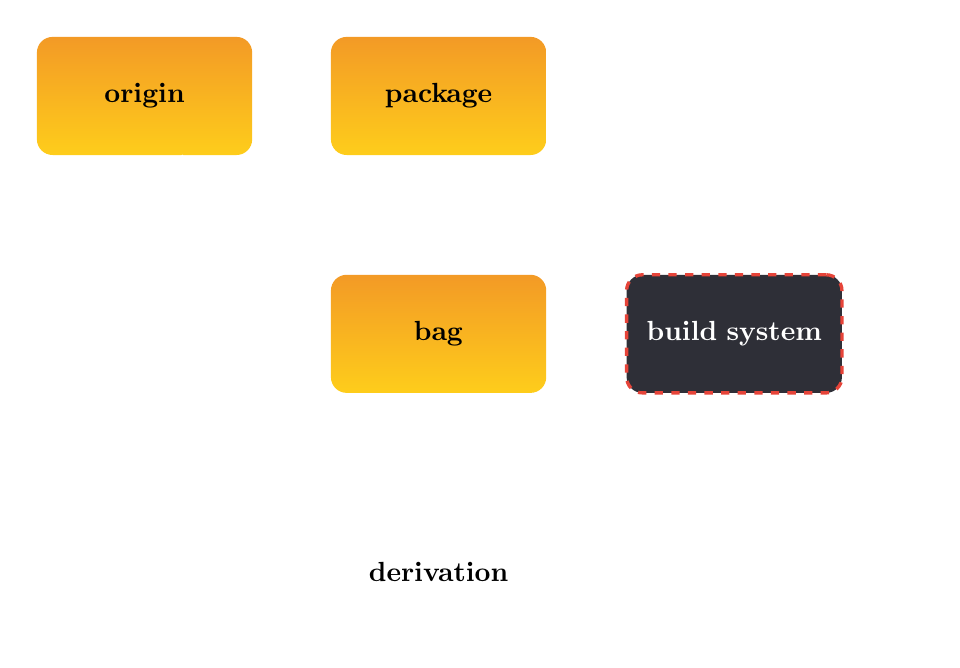
\begin{tikzpicture}[hilevel/.style = {
                        rectangle, text width=25mm, text centered,
                        rounded corners=2mm, minimum height=15mm,
                        top color=guixorange1,
                        bottom color=guixyellow,
                        text=black
                      },
                      buildsys/.style = {
                        rectangle, text width=25mm, text centered,
                        rounded corners=2mm, minimum height=15mm,
                        very thick, dashed, fill=guixdarkgrey,
                        text=white, text opacity=1, draw=guixred2
                      },
                      drv/.style = {
                        rectangle, text width=25mm, text centered,
                        rounded corners=2mm, minimum height=15mm,
                        fill=white, text=black
                      }]
    \matrix[row sep=15mm, column sep=1cm] {
      \node(package)[hilevel] {\textbf{origin}}; &
      \node(origin)[hilevel] {\textbf{package}}; &
      &
      \\

      & \node(bag) [hilevel] {\textbf{bag}}; &
      \node(buildsys) [buildsys] {\textbf{build system}}; &
      \\

      & \node(derivation) [drv] { \textbf{derivation} };
      & &
      \\
    };

    % bag/derivation are inverted!  XXX
    \path[->, very thick, draw=white, sloped] (origin) edge (bag);
    \path[->, very thick, draw=white] (bag) edge (derivation);
    \path[->, very thick, draw=white] (package) edge (derivation);
  \end{tikzpicture}
\end{frame}

\begin{frame}[fragile]{}
  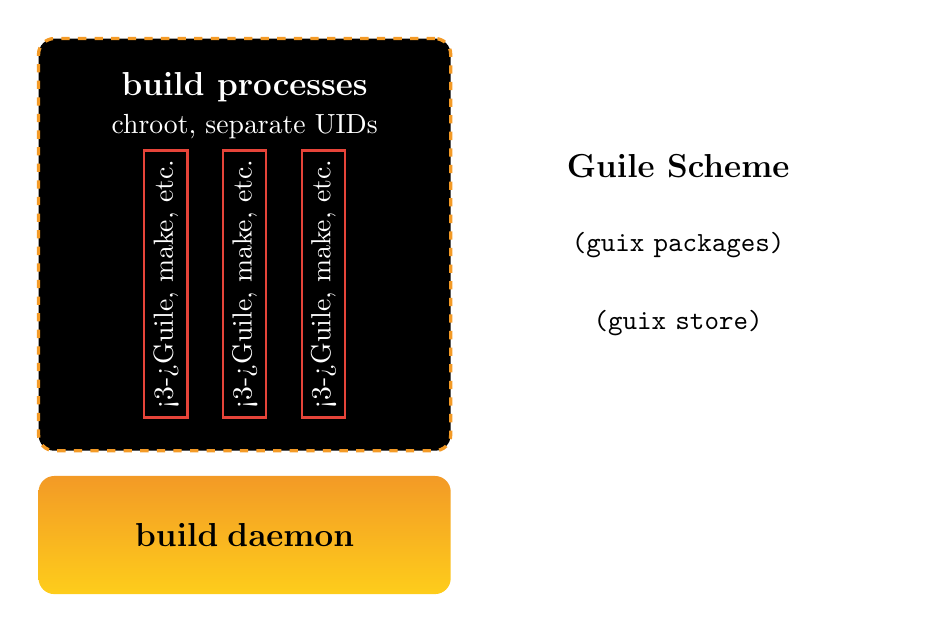
\begin{tikzpicture}[tools/.style = {
                        text width=35mm, minimum height=4cm,
                        text centered,
                        rounded corners=2mm,
                        fill=white, text=black
                      },
                      tool/.style = {
                        fill=white, text=black, text width=3cm,
                        text centered
                      },
                      daemon/.style = {
                        rectangle, text width=50mm, text centered,
                        rounded corners=2mm, minimum height=15mm,
                        top color=guixorange1,
                        bottom color=guixyellow,
                        text=black
                      },
                      builders/.style = {
                        draw=guixorange1, very thick, dashed,
                        fill=black, text=white, text width=5cm,
                        rounded corners=2mm,
                      },
                      builder/.style = {
                        draw=guixred2, thick, rectangle,
                        fill=black, text=white,
                        rotate=90
                      }]
    \matrix[row sep=3mm, column sep=1cm] {
      \node(builders)[builders, text height=5cm]{}
          node[fill=black, text=white] at (0, 2) {\large{\textbf{build processes}}}
          node[fill=black, text=white] at (0, 1.5) {chroot, separate UIDs}
          node[builder, onslide=<1-2>{black}] at (-1,-0.5) {\alert<3->{Guile}, make, etc.}
          node[builder, onslide=<1-2>{black}] at ( 0,-0.5) {\alert<3->{Guile}, make, etc.}
          node[builder, onslide=<1-2>{black}] at ( 1,-0.5) {\alert<3->{Guile}, make, etc.}; &
      \node[tools]{}
          node[fill=white, text=black] at (0, 1) {\large{\textbf{Guile Scheme}}}
          node[tool] at (0, 0) {\texttt{(guix packages)}}
          node(client)[tool] at (0, -1) {\texttt{(guix store)}};
      \\

      \node(daemon)[daemon]{\large{\textbf{build daemon}}}; &
      &
      \\
    };
  \end{tikzpicture}

  \begin{tikzpicture}[overlay]
    \path[very thick, draw=guixorange1]<2->
      (client.south) edge [out=-90, in=0, ->] node[below, sloped]{RPCs} (daemon.east);
    \path[->, very thick, draw=guixorange1]<3->
      (daemon) edge (builders);
  \end{tikzpicture}
\end{frame}

%% TODO: Add LMI picture with ``Why stop here?''.

\begin{frame}[fragile]
  \begin{semiverbatim}
    \small{
(\alert{operating-system}
  (host-name "schememachine")
  (timezone "Japan")
  (locale "ja_JP.utf8")
  (bootloader (grub-configuration (device "/dev/sda")))
  (file-systems (cons (\alert{file-system}
                        (device "my-root")
                        (title 'label)
                        (mount-point "/")
                        (type "ext4"))
                      %base-file-systems))
  (users (cons (\alert{user-account}
                 (name "alice")
                 (group "users")
                 (home-directory "/home/alice"))
               %base-user-accounts))
  (services (cons* (dhcp-client-service)
                   (lsh-service #:port-number 2222)
                   %base-services)))
    }
  \end{semiverbatim}
\end{frame}

\begin{frame}[fragile]
  \begin{overlayarea}{\textwidth}{8cm}
  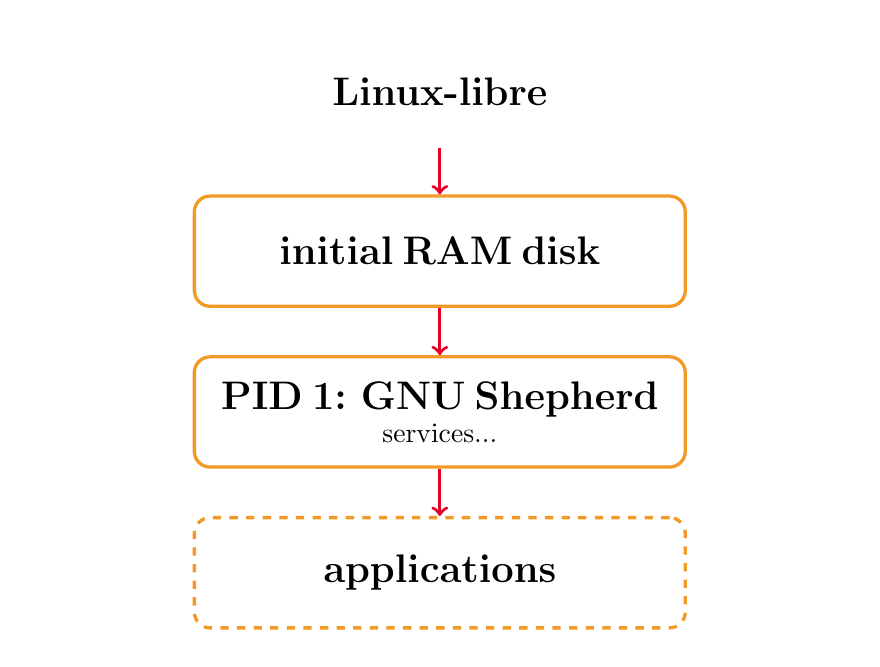
\begin{tikzpicture}[kernel/.style = {
                        text width=10cm, minimum height=1.4cm,
                        text centered,
                        rounded corners=2mm,
                        fill=white, text=black
                      },
                      userland/.style = {
                        draw=guixorange1, very thick,
                        fill=white, text=black, text width=6cm,
                        rounded corners=2mm, minimum height=1.4cm,
                        text centered
                      }]
    \matrix[row sep=6mm, column sep=1cm] {
      \node(kernel)[kernel]{\textbf{\Large{Linux-libre}}};
      \\

      \node<2->(initrd)[userland]{\textbf{\Large{initial RAM disk}}};
      \\

      \node<4->(shepherd)[userland]{\textbf{\Large{PID 1: GNU Shepherd}}
        \\ services...};
      \\

      \node<6->(user)[userland, dashed]{\textbf{\Large{applications}}};
      \\
    };

    \path[->, very thick, draw=guixred1]<2->
      (kernel) edge (initrd);
    \path[->, very thick, draw=guixred1]<4->
      (initrd) edge (shepherd);
    \path[->, very thick, draw=guixred1]<6->
      (shepherd) edge (user);
    
  \end{tikzpicture}
  \end{overlayarea}

  \begin{tikzpicture}[overlay,
                      guile/.style = {
                         fill=guixyellow, text=black, rotate=30,
                         rounded corners=4mm, text width=3cm,
                         opacity=.75, text opacity=1, text centered,
                         minimum height=1.3cm
                      }]
    \node<3->(labelinitrd) [guile] at (initrd.east) {%
      \Large{Guile}
    };
    \node<5->(labelinitrd) [guile] at (shepherd.east) {%
      \Large{Guile}
    };
  \end{tikzpicture}
\end{frame}

\setbeamercolor{normal text}{bg=guixblue2}
\begin{frame}
  \Huge{\textbf{Code staging.}}
\end{frame}
\setbeamercolor{normal text}{fg=white,bg=black}

\begin{frame}[fragile]{}
  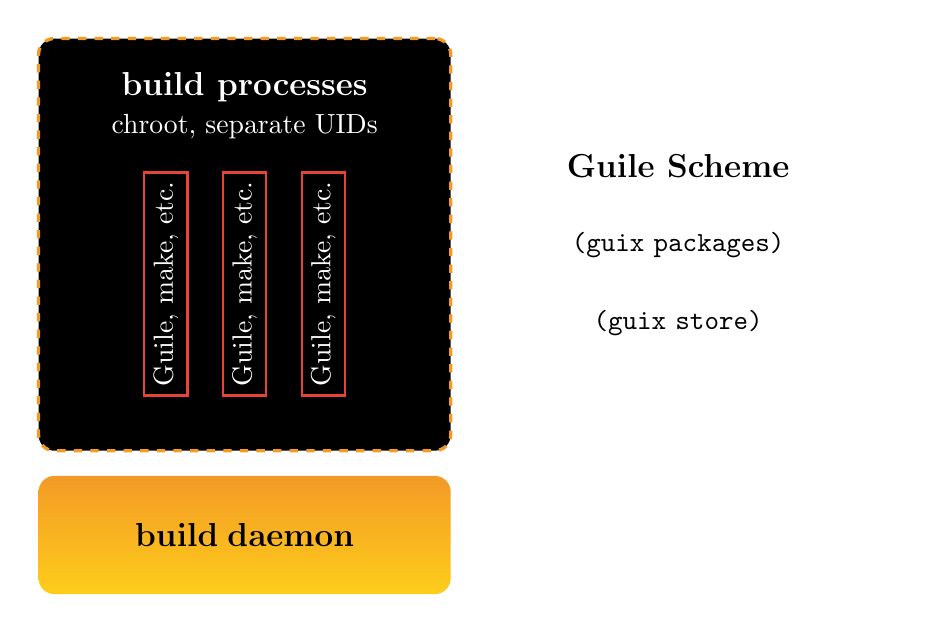
\begin{tikzpicture}[tools/.style = {
                        text width=35mm, minimum height=4cm,
                        text centered,
                        rounded corners=2mm,
                        fill=white, text=black
                      },
                      tool/.style = {
                        fill=white, text=black, text width=3cm,
                        text centered
                      },
                      daemon/.style = {
                        rectangle, text width=50mm, text centered,
                        rounded corners=2mm, minimum height=15mm,
                        top color=guixorange1,
                        bottom color=guixyellow,
                        text=black
                      },
                      builders/.style = {
                        draw=guixorange1, very thick, dashed,
                        fill=black, text=white, text width=5cm,
                        rounded corners=2mm,
                      },
                      builder/.style = {
                        draw=guixred2, thick, rectangle,
                        fill=black, text=white,
                        rotate=90
                      }]
    \matrix[row sep=3mm, column sep=1cm] {
      \node(builders)[builders, text height=5cm]{}
          node[fill=black, text=white] at (0, 2) {\large{\textbf{build processes}}}
          node[fill=black, text=white] at (0, 1.5) {chroot, separate UIDs}
          node[builder] at (-1,-0.5) {\alert{Guile}, make, etc.}
          node[builder] at ( 0,-0.5) {\alert{Guile}, make, etc.}
          node[builder] at ( 1,-0.5) {\alert{Guile}, make, etc.}; &
      \node[tools]{}
          node[fill=white, text=black] at (0, 1) {\large{\textbf{Guile Scheme}}}
          node[tool] at (0, 0) {\texttt{(guix packages)}}
          node(client)[tool] at (0, -1) {\texttt{(guix store)}};
      \\

      \node(daemon)[daemon]{\large{\textbf{build daemon}}}; &
      &
      \\
    };
  \end{tikzpicture}

  \begin{tikzpicture}[overlay]
    \path[very thick, draw=guixorange1]
      (client.south) edge [out=-90, in=0, ->] node[below, sloped]{RPCs} (daemon.east);
    \path[->, very thick, draw=guixorange1]
      (daemon) edge (builders);
  \end{tikzpicture}
\end{frame}

\begin{frame}[fragile]{Staging: take \#1}
  \vspace{-0.2cm}
  \begin{semiverbatim}
(define \alert{build-exp}
  ;; \textsl{Build-side code.}
  '(symlink (assoc-ref \alert{%build-inputs} "coreutils")
            \alert{%output}))

;; \textsl{... with unhygienic global variable:}
;; (define %build-inputs
;;   '(\only<1>{("coreutils" . "/gnu/store/\textrm{...}-coreutils-8.25")}\only<2>{}))

\uncover<1>{(define \alert{inputs}
  ;; \textsl{What goes into the chroot.}
  `(("coreutils" ,coreutils)))}

(build-expression->derivation store
                              "symlink-to-coreutils"
                              \alert{build-exp}
                              \uncover<1>{#:inputs \alert{inputs}})
\pause
  \end{semiverbatim}
\end{frame}

\screenshot{images/poor-staging-good-staging}

\begin{frame}[fragile]{Take \#2: G-expressions}
  \begin{semiverbatim}
(define \alert{build-exp}
  ;; \textsl{First-class object that carries info}
  ;; \textsl{about its dependencies.}
  (\alert{gexp} (symlink (\alert{ungexp} coreutils)
                 (\alert{ungexp output}))))

;; \textsl{Leads to a build script like:}
;; (symlink "/gnu/store/123\textrm{...}-coreutils-8.25"
;;          (getenv "out"))

(gexp->derivation "symlink-to-coreutils" \alert{build-exp})
  \end{semiverbatim}
\end{frame}

\begin{frame}[fragile]{Take \#2: G-expressions}
  \begin{semiverbatim}
(define \alert{build-exp}
  ;; \textsl{First-class object that carries info}
  ;; \textsl{about its dependencies.}
  \alert{#~}(symlink \alert{#$}coreutils \alert{#$output}))

;; \textsl{Leads to a build script like:}
;; (symlink "/gnu/store/\only<1>{123}\only<2>{h8a}\textrm{...}-coreutils-8.25"
;;          (getenv "out"))

(gexp->derivation "symlink-to-coreutils" \alert{build-exp}\only<1>{)}
                  \only<2>{\alert{#:system} "i686-linux")}
  \end{semiverbatim}
\end{frame}

\begin{frame}[fragile]{Cross-Compilation}
  \begin{semiverbatim}
(gexp->derivation "vi"
   \alert{#~}(begin
       (mkdir \alert{#$output})
       (system* (string-append \alert{#+}coreutils "/bin/ln")
                "-s"
                (string-append \alert{#$}emacs "/bin/emacs")
                (string-append \alert{#$}output "/bin/vi")))
\only<2>{   \alert{#:target} "mips64el-linux-gnu"})

;; \textsl{Yields:}
;; (begin
;;   (mkdir (getenv "out"))
;;   (system* (string-append "/gnu/store/123\textrm{...}" "/bin/ln")
;;            "-s"
;;            (string-append "/gnu/store/\only<1>{345}\only<2>{\alert{9ab}}\textrm{...}" \textrm{...})
;;            (string-append "/gnu/store/\only<1>{567}\only<2>{\alert{fc2}}\textrm{...}" \textrm{...})))
  \end{semiverbatim}
\end{frame}

\begin{frame}[fragile]{Modules}
  \begin{semiverbatim}
(define \alert{build-exp}
\uncover<2>{  ;; \textsl{Compile (guix build utils) and add it}
  ;; \textsl{to the chroot.}
  (\alert{with-imported-modules} '((guix build utils))}
    \alert{#~}(begin
        (\alert{use-modules} (guix build utils))
        (mkdir-p (string-append \alert{#$output} "/bin"))\only<2>{)}

(gexp->derivation "empty-bin-dir" build-exp)
\only<1>{;; \textsl{ERROR: (guix build utils) not found!}}
  \end{semiverbatim}
\end{frame}

\begin{frame}[fragile]{Modules \& Scripts}
  \begin{semiverbatim}
(define \alert{script}
  (\alert{with-imported-modules} (source-module-closure
                          '((guix build gremlin)))
    \alert{#~}(begin
        (\alert{use-modules} (guix build gremlin)
                     (ice-9 match))

        (match (command-line)
          ((command argument)
           (validate-needed-in-runpath argument))))))

(gexp->script "check-runpath" script)
  \end{semiverbatim}
\end{frame}


\begin{frame}[fragile]{Modules \& Initial RAM Disk}
  \begin{semiverbatim}
(expression->initrd
 (\alert{with-imported-modules} (source-module-closure
                         '((gnu build linux-boot)
                           (guix build utils)))
   \alert{#~}(begin
       (\alert{use-modules} (gnu build linux-boot)
                    (guix build utils))

       (boot-system #:mounts '#$file-systems
                    #:linux-modules '#$linux-modules
                    #:linux-module-directory '#$kodir)))
  \end{semiverbatim}
\end{frame}

\begin{frame}[fragile]{Defining ``Compilers''}
  \begin{semiverbatim}
    \small{
(\alert{define-gexp-compiler} (package-compiler (package \alert{<package>})
                                        system target)
  ;; \textsl{Return a derivation to build PACKAGE.}
  (if target
      (package->cross-derivation package target system)
      (package->derivation package system)))
    }
\pause
(define-record-type \alert{<plain-file>}
  (plain-file name content)
  \textrm{...})

(\alert{define-gexp-compiler} (plain-file-compiler (file \alert{<plain-file>})
                                           system target)
  ;; \textsl{"Compile" FILE by adding it to the store.}
  (match file
    (($ \alert{<plain-file>} name content)
     (text-file name content))))
  \end{semiverbatim}
\end{frame}

\begin{frame}[fragile]{Compilers \& ``Expanders''}
  \begin{semiverbatim}
\alert{#~}(string-append \alert{#$}coreutils "/bin/ls")

;; \textsl{Yields:}
;; (string-append "/gnu/store/\textrm{...}" "/bin/ls")
\pause
(file-append coreutils "/bin/ls")

;; \textsl{Yields:}
;; "/gnu/store/\textrm{...}/bin/ls"
  \end{semiverbatim}
\end{frame}

\begin{frame}[fragile]{Implementation}
  \Large{
    \begin{itemize}
    \item \texttt{gexp} macro
    \item \texttt{<gexp>} record type
    \item \texttt{gexp->sexp} linear in the number of \texttt{ungexp}
    \end{itemize}
  }
\end{frame}

\begin{frame}[fragile]{Limitations}
  \begin{itemize}
    \item \highlight{hygiene}, oh my!
    \item \highlight{modules} in scope?
    \item \highlight{serialization} of non-primitive data types?
    \item cross-stage \highlight{debugging info} à la Hop?
  \end{itemize}
\end{frame}

\setbeamercolor{normal text}{bg=guixdarkgrey,fg=guixred3}
\begin{frame}[fragile]
  \Huge{Related Work}
\end{frame}
\setbeamercolor{normal text}{fg=white,bg=black}

\begin{frame}[fragile]{\texttt{syntax-case}}
  \begin{itemize}
  \item gexps similar in spirit to syntax objects
  \item ... but staging with gexps is not referentially transparent
  \end{itemize}

  \vfill{}
  \small{
    \textit{Writing Hygienic Macros in Scheme with Syntax-Case}, R. Kent
    Dybvig, 1992
  }
\end{frame}

\begin{frame}[fragile]{MetaScheme}

  \begin{itemize}
  \item referentially transparent (``hygienic'') staging
  \item {... but PoC is simplistic
    \begin{itemize}
    \item modules in scope?
    \item how to determine which forms introduce bindings?
    \end{itemize}}
  \end{itemize}

  \vfill{}
  \small{
    \textit{MetaScheme, or untyped MetaOCaml},
    \url{http://okmij.org/ftp/meta-programming/}, O. Kiselyov, 2008
  }
\end{frame}

\begin{frame}[fragile]{Hop}

  \begin{semiverbatim}
(define-service (shello6 x)
  (<HTML>
    (<BODY>
      :onclick \alert{~}(with-hop (\alert{$}(service ()
                              (format "Bonjour ~a" x)))
                  (lambda (v) (alert v)))
      "Hello!")))
  \end{semiverbatim}
\end{frame}

\begin{frame}[fragile]{Hop}
  \begin{itemize}
  \item staged code is \highlight{JavaScript}, not Scheme
  \item programmers can express \highlight{modules in scope} for staged
    code
  \item{ \texttt{\~} and \texttt{\$} implemented as compiler magic
    \begin{itemize}
    \item \texttt{\~} expressions are not first-class objects
    \end{itemize}
  }
  \end{itemize}

  \vfill{}
  \small{
    \textit{A Multi-Tier Semantics for Hop}, Serrano and Queinnec, 2010
  }
\end{frame}

\begin{frame}[fragile]
  \frametitle{Nix language}

  \small{
    \begin{semiverbatim}
\only<2->{\alert{let} dep = }\tikz[baseline]{\node[anchor=base](funcall){\alert{derivation}};} \{
  name = "foo";
  system = "x86\_64-linux";
  builder = "\alert{\$\{./static-bash\}}";
  args = [ "-c" "echo hello > "\tikz[baseline]{\node[anchor=base](outvar){$out};}" ];
\tikz[baseline]{\node[anchor=base](args){\}};}\uncover<2->{;}\uncover<2->{ in \alert{derivation} \{
  name = "bar";
  system = "x86\_64-linux";
  builder = "\alert{\$\{./static-bash\}}";
  args = [ "-c"
    '' mkdir -p "$out"
       ln -s "\tikz[baseline]{\node[anchor=base](strinterp){\alert{$\{dep\}}};}/some-result" "\$out/my-result"
    '' ];
  PATH = "\$\{coreutils\}/bin";
\} }
    \end{semiverbatim}
  }

  \only<2>{
    \begin{textblock}{7}(5,14)
      \tikz \node[fill=white, text=black](labelstrinterp){expands to \texttt{/nix/store/\textrm{...}-foo}};
    \end{textblock}

    \begin{tikzpicture}[overlay]
      \path[->](labelstrinterp) edge (strinterp);
    \end{tikzpicture}
  }
\end{frame}

\begin{frame}[fragile]{Nix language}
  \begin{itemize}
  \item has \highlight{string interpolation}
  \item strings retain info about their \highlight{dependencies}
  \item built into the interpreter
  \end{itemize}

  \vfill{} \small{ \textit{NixOS: A Purely Functional Linux
      Distribution}, Dolstra and Löh, 2008 }
\end{frame}

\screenshot{images/nix-shell-escapes}

\setbeamercolor{normal text}{bg=guixblue2}
\begin{frame}
  \Huge{\textbf{Wrap up.}}
\end{frame}
\setbeamercolor{normal text}{fg=white,bg=black}

\begin{frame}[fragile]{Summary}
  \Large{
    \begin{itemize}
    \item Guix provides \highlight{functional OS deployment}
    \item it's a \highlight{Scheme library and toolbox}
    \item it's a \highlight{multi-tier Scheme system}
    \end{itemize}
  }
\end{frame}

\begin{frame}[fragile]{Lots of other niceties!}
  \Large{
    \begin{itemize}
    \item \highlight{system service} architecture
    \item ... and services written in Scheme (Shepherd, mcron)
    \item \highlight{Emacs} integration
    \item \highlight{whole-system test suite} (staging!)
    \item \highlight{distributed deployment} with Guile-SSH (staging!)
    \item ...
    \end{itemize}
  }
\end{frame}

\begin{frame}[plain]
  \begin{tikzpicture}[remember picture, overlay]
    \node [at=(current page.center), inner sep=0pt]
          {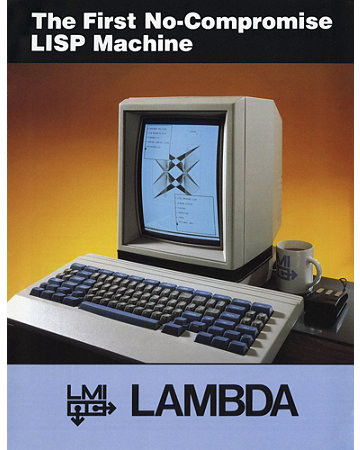
\includegraphics[height=\paperheight]{images/lmi-machine}};
  \end{tikzpicture}
\end{frame}

\begin{frame}{Join us now, share the parens!}
  \vspace{0.7cm}
  \Large{
    \begin{itemize}
    \item \textbf{install the distribution}
    \item \textbf{use it}, report bugs, add packages
    \item share your \textbf{ideas}!
    \end{itemize}
  }
\end{frame}

%%%%%%%%%%%%%%%%%%%%%%%%%%%%%%%%%%%%%%%%%%%%%%%%%%%%%%%%%%%%%%%%%%%%%%%%%%%%%%
\begin{frame}[plain]

\vfill{
  \vspace{2.5cm}
  \center{
\includegraphics[width=0.3\textwidth]{images/GuixSD}}\\[1.0cm]
  \texttt{ludo@gnu.org}\hfill{\alert{\url{http://gnu.org/software/guix/}}}
}

\end{frame}

\begin{frame}{}

  \begin{textblock}{12}(2, 8)
    \tiny{
      Copyright \copyright{} 2010, 2012--2016 Ludovic Courtès \texttt{ludo@gnu.org}.\\[3.0mm]
      GNU GuixSD logo, CC-BY-SA 4.0, \url{http://gnu.org/s/guix/graphics}

      Copyright of other images included in this document is held by
      their respective owners.
      \\[3.0mm]
      This work is licensed under the \alert{Creative Commons
        Attribution-Share Alike 3.0} License.  To view a copy of this
      license, visit
      \url{http://creativecommons.org/licenses/by-sa/3.0/} or send a
      letter to Creative Commons, 171 Second Street, Suite 300, San
      Francisco, California, 94105, USA.
      \\[2.0mm]
      At your option, you may instead copy, distribute and/or modify
      this document under the terms of the \alert{GNU Free Documentation
        License, Version 1.3 or any later version} published by the Free
      Software Foundation; with no Invariant Sections, no Front-Cover
      Texts, and no Back-Cover Texts.  A copy of the license is
      available at \url{http://www.gnu.org/licenses/gfdl.html}.
      \\[2.0mm]
      % Give a link to the 'Transparent Copy', as per Section 3 of the GFDL.
      The source of this document is available from
      \url{http://git.sv.gnu.org/cgit/guix/maintenance.git}.
    }
  \end{textblock}
\end{frame}

\end{document}

% Local Variables:
% coding: utf-8
% comment-start: "%"
% comment-end: ""
% ispell-local-dictionary: "american"
% compile-command: "rubber --pdf talk.tex"
% End:
